% Provenance (never printed): see sources/outline_sources.md and sources/book1/BRIEFS.md (g9/05).
\chapter{Randomness and Simulation}\label{ch:g9:randomness-and-simulation}

Tom throws a die 60 times and gets only four sixes. He expected about ten. Is
the die unfair, or is it just luck? Throwing a real die thousands of times would
take days; a \omterm{def:g4:programs-and-operating-system:program}{program} throws it a million times in a second. This chapter makes
the \omterm{def:g1:what-is-a-computer:computer}{computer} play dice, shows where its ``random'' numbers come from, and uses
them to answer questions that are hard to work out by hand.

\begin{recall}
A \omterm{def:g7:lists:list}{list} keeps \omterm{def:g6:variables-and-input:value}{values} in order (\cref{ch:g7:lists}); a \omterm{def:g8:dictionaries:dictionary}{dictionary} can count how
often each \omterm{def:g6:variables-and-input:value}{value} appears (\cref{ch:g8:dictionaries}). From mathematics: the
probability of an event is a number from 0 to 1; with a fair die, each face has
probability $1/6$; the frequency of an event is the number of times it happened
divided by the number of tries; the area of a disc of radius $r$ is $\pi r^2$.
\end{recall}

\begin{omfigure}
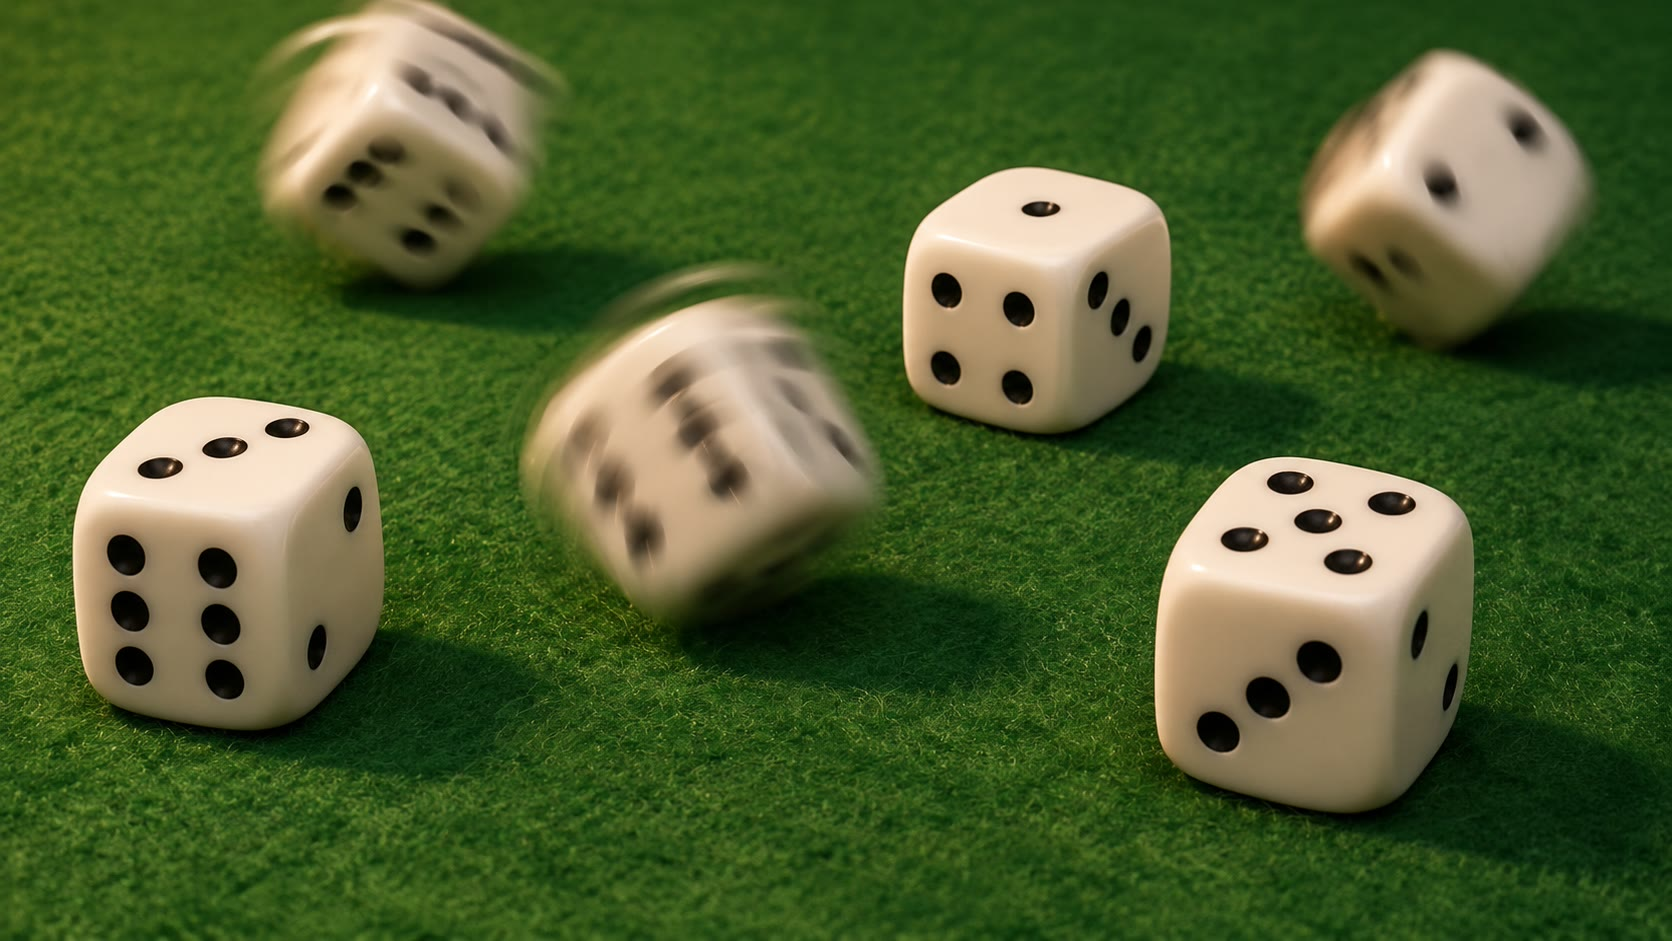
\includegraphics[width=0.5\linewidth, trim=0 0 492 0, clip]{images/book1/ai/g9-randomness-and-simulation-dice.jpg}

{\small Dice rolling on a table. Which face comes up depends on how they are
thrown, too finely to predict: that is what makes them a game of chance.}
\end{omfigure}

\section{Pseudo-random numbers and the seed}

A \omterm{def:g1:what-is-a-computer:computer}{computer} follows its \omterm{def:g1:instructions-in-order:instruction}{instructions} exactly: given the same \omterm{def:g1:instructions-in-order:instruction}{instructions}, it
does the same thing. So where do random numbers come from? From a rule that
mixes a number so thoroughly that the results \emph{look} random.

\begin{definition}[Pseudo-random number generator]\label{def:g9:randomness-and-simulation:prng}
A \emph{pseudo-random number generator}\index{pseudo-random number generator}
is a rule that keeps a hidden \emph{state} (one number, or a \omterm{def:g7:lists:list}{list} of numbers),
changes it at each step and reads the next number from it, so that the
sequence looks random although it is fully determined.
\end{definition}

\begin{definition}[Seed]\label{def:g9:randomness-and-simulation:seed}
The \emph{seed}\index{seed} of a generator is the number its state starts from. The
same seed always gives the same sequence.
\end{definition}

A tiny generator multiplies by 5, adds 3 and keeps the remainder by 16:

\omcode{code/grade-9/05-randomness-and-simulation/listings/tiny_generator.py}{1}{12}{A
tiny generator, run until it repeats.}\label{lst:g9:randomness-and-simulation:tiny}

\Needspace*{6\baselineskip}
\omoutput{code/grade-9/05-randomness-and-simulation/outputs/tiny_generator.txt}{All
sixteen numbers from 0 to 15, then the same again.}\label{out:g9:randomness-and-simulation:tiny}

\begin{omfigure}
\begin{tikzpicture}
  \foreach \v [count=\i from 0] in {7, 6, 1, 8, 11, 10, 5, 12, 15, 14, 9, 0, 3, 2, 13, 4} {
    \node[circle, draw=ocInk, fill=ocBlue!15, minimum size=6.5mm, inner sep=0pt,
      font=\small] (n\i) at ({90 - \i * 22.5}:2.6cm) {\v};
  }
  \foreach \i [evaluate=\i as \j using {int(mod(\i + 1, 16))}] in {0,...,15} {
    \draw[-{Stealth[length=1.6mm]}, ocBlue] (n\i) to[bend left=12] (n\j);
  }
  \node[draw=ocRed, very thick, circle, minimum size=7.5mm] at (n0) {};
  \node[font=\small, align=center] at (0,0) {$x \to (5x + 3) \bmod 16$\\ seed 7};
\end{tikzpicture}

{\small The tiny generator's sixteen numbers, in the order it gives them. After
the sixteenth, it is back to its \omterm{def:g9:randomness-and-simulation:seed}{seed} (red) and goes round again.}
\end{omfigure}

Here the state is the number itself. The numbers jump around, but they come
back after 16: the generator can only produce 16 different \omterm{def:g6:variables-and-input:value}{values}, and once
its state comes back, everything after it repeats. Python's generator works on
the same principle, but its state is a \omterm{def:g7:lists:list}{list} of hundreds of numbers: a
number it gives can come back without the sequence repeating, and the cycle of
its state is far beyond anything a \omterm{def:g4:programs-and-operating-system:program}{program} could ever use.

% ledger: g9:python-mersenne-twister
Python's module \code{random} gives the tools. \code{random.seed(n)} sets the
\omterm{def:g9:randomness-and-simulation:seed}{seed}; \code{random.randint(a, b)} returns a whole number from \code{a} to
\code{b}, both included; \code{random.random()} a decimal number from 0 up to
(but not including) 1; \code{random.choice(items)} one \omterm{def:g7:lists:list}{item} of a \omterm{def:g7:lists:list}{list};
\code{random.shuffle(items)} mixes a \omterm{def:g7:lists:list}{list} in place. Its generator, called the
Mersenne Twister, repeats only after $2^{19937} - 1$ numbers. Because it is
completely determined by its \omterm{def:g9:randomness-and-simulation:seed}{seed}, its documentation warns that it must never be
used for secrets, such as \omterm{def:g5:networks-first-look:password}{passwords}; Python has another module,
\code{secrets}, for those.

\Needspace*{12\baselineskip}
\omcode{code/grade-9/05-randomness-and-simulation/listings/seed_demo.py}{1}{9}{The
same \omterm{def:g9:randomness-and-simulation:seed}{seed}, the same numbers.}\label{lst:g9:randomness-and-simulation:seed}

\Needspace*{8\baselineskip}
\omoutput{code/grade-9/05-randomness-and-simulation/outputs/seed_demo.txt}{The first
two lines are the same.}\label{out:g9:randomness-and-simulation:seed}

Every \omterm{def:g4:programs-and-operating-system:program}{program} of this chapter sets a \omterm{def:g9:randomness-and-simulation:seed}{seed} at the start. That is why each \omterm{def:g1:what-is-a-computer:input}{output}
printed in this book comes out exactly the same every time it is run, on any
\omterm{def:g1:what-is-a-computer:computer}{computer}. Without \code{random.seed}, Python takes a \omterm{def:g9:randomness-and-simulation:seed}{seed} from the \omterm{def:g4:programs-and-operating-system:os}{operating
system}'s sources of randomness, or from the clock, and each run gives new
numbers.

\section{Simulating dice, coins and draws}

\begin{definition}[Simulation]\label{def:g9:randomness-and-simulation:simulation}
A \emph{simulation}\index{simulation} is a \omterm{def:g4:programs-and-operating-system:program}{program} that imitates a real process,
here one that involves chance, so that it can be run many times quickly.
\end{definition}

\omcode{code/grade-9/05-randomness-and-simulation/listings/dice.py}{1}{15}{A die, two
dice and a bag of marbles.}\label{lst:g9:randomness-and-simulation:dice}

\Needspace*{7\baselineskip}
\omoutput{code/grade-9/05-randomness-and-simulation/outputs/dice.txt}{Twenty throws
of one die, ten of two.}\label{out:g9:randomness-and-simulation:dice}

Two dice are two separate calls to \code{randint}, added: \code{randint(2, 12)}
would be wrong, because it makes every sum equally likely, and with real dice a
7 is far more frequent than a 2. A deck of cards is a \omterm{def:g7:lists:list}{list}, mixed by
\code{shuffle}:

\omcode{code/grade-9/05-randomness-and-simulation/listings/deck.py}{1}{12}{A deck,
shuffled, and a hand of five.}\label{lst:g9:randomness-and-simulation:deck}

\Needspace*{7\baselineskip}
\omoutput{code/grade-9/05-randomness-and-simulation/outputs/deck.txt}{The hand is the
first five cards of the shuffled deck.}\label{out:g9:randomness-and-simulation:deck}

\section{Frequencies settle near the probability}

Back to Tom's question. This \omterm{def:g4:programs-and-operating-system:program}{program} throws a die 10 times, then 20, 50, and so
on up to 100,000 times, and prints the frequency of a six each time:

\omcode{code/grade-9/05-randomness-and-simulation/listings/frequencies.py}{1}{12}{The
frequency of a six, for more and more throws.}\label{lst:g9:randomness-and-simulation:frequencies}

\omoutput{code/grade-9/05-randomness-and-simulation/outputs/frequencies.txt}{From 0.1
to 0.2 at first, then close to 0.1667.}\label{out:g9:randomness-and-simulation:frequencies}

\begin{omfigure}
\begin{tikzpicture}
  \begin{axis}[width=11cm, height=5.2cm, xmode=log, xmin=7, xmax=150000,
      ymin=0.08, ymax=0.22, xlabel={number of throws}, ylabel={frequency of a six},
      yticklabel style={/pgf/number format/fixed, /pgf/number format/precision=2},
      grid=major, grid style={black!10}]
    \addplot[ocRed, thick, dashed, domain=7:150000, samples=2] {1/6};
    \addplot[ocBlue, thick, mark=*, mark size=1.6pt] table[x=throws, y=frequency]
      {code/grade-9/05-randomness-and-simulation/figures/out/frequency.dat};
    \node[anchor=south east, font=\small, ocRed] at (axis cs:120000,0.168) {$1/6$};
  \end{axis}
\end{tikzpicture}

{\small The frequency of a six from \cref{out:g9:randomness-and-simulation:frequencies};
each step to the right multiplies the number of throws by 10. Far from $1/6$ for
a few throws, close to it for many.}
\end{omfigure}

With a few dozen throws, the frequency wanders: 0.10, 0.15, 0.20. With tens of
thousands, it stays within a few thousandths of $1/6$. Four sixes in 60 throws
is a frequency of 0.067, lower than any point of the chart: unusual for a fair
die, but with so few throws, frequencies wander a lot, and a fair die does give
such a result now and then. To decide, Tom needs many more throws: with a few
thousand, a fair die stays close to $1/6$, and a die that really favours some
faces shows it.

\section{A random walk}

A token stands at 0 on a number line. At each step a coin is tossed: heads, it
moves one place right; tails, one place left. Where is it after 100 steps?

\omcode{code/grade-9/05-randomness-and-simulation/listings/random_walk.py}{1}{22}{A
walk of 100 steps, left or right by a coin.}\label{lst:g9:randomness-and-simulation:walk}

\Needspace*{7\baselineskip}
\omoutput{code/grade-9/05-randomness-and-simulation/outputs/random_walk.txt}{One
walk.}\label{out:g9:randomness-and-simulation:walk}

\begin{omfigure}
\begin{tikzpicture}
  \begin{axis}[width=11cm, height=4.6cm, xmin=0, xmax=100, ymin=-8, ymax=13,
      xlabel={step}, ylabel={position}, grid=major, grid style={black!10}]
    \addplot[black!40, domain=0:100, samples=2] {0};
    \addplot[ocBlue, thick, const plot] table[x=step, y=position]
      {code/grade-9/05-randomness-and-simulation/figures/out/walk.dat};
  \end{axis}
\end{tikzpicture}

{\small The walk of \cref{out:g9:randomness-and-simulation:walk}, step by step: it
goes down to $-6$ early on, then drifts up and ends at 10.}
\end{omfigure}

The \omterm{def:g7:functions:function}{function} \code{walk} returns the whole path, so the \omterm{def:g4:programs-and-operating-system:program}{program} can ask
questions about it afterwards: the end, the farthest point on each side. Run
with another \omterm{def:g9:randomness-and-simulation:seed}{seed}, the walk ends somewhere else entirely. Exercise
\ref{exo:g9:randomness-and-simulation:12} asks how often it comes back to 0.

\section{Estimating by simulation}

\begin{method}[Estimation by simulation]\label{met:g9:randomness-and-simulation:estimate}
To estimate\index{estimation by simulation} the probability of an event, simulate
the random process many times, count how often the event happens, and divide by
the number of tries. The more tries, the closer the frequency usually is to the
probability.
\end{method}

What is the chance that two dice add up to 7? The \omterm{def:g4:programs-and-operating-system:program}{program} simulates 100,000
throws, then counts exactly: of the 36 pairs of faces, 6 add up to 7.

\omcode{code/grade-9/05-randomness-and-simulation/listings/sum_seven.py}{1}{16}{A
seven with two dice: simulated and exact.}\label{lst:g9:randomness-and-simulation:seven}

\Needspace*{6\baselineskip}
\omoutput{code/grade-9/05-randomness-and-simulation/outputs/sum_seven.txt}{The two
agree to about a thousandth.}\label{out:g9:randomness-and-simulation:seven}

\omterm{def:g9:randomness-and-simulation:simulation}{Simulation} can even estimate $\pi$. Throw points at random in a square of side
1. The quarter of a disc of radius 1 covers $\pi / 4$ of the square, so about
$\pi / 4$ of the points fall inside it, where $x^2 + y^2 \le 1$. Four times the
fraction of points inside estimates $\pi$.

\begin{omfigure}
\begin{tikzpicture}
  \begin{axis}[width=6cm, height=6cm, xmin=0, xmax=1, ymin=0, ymax=1,
      axis equal image, xtick={0,1}, ytick={0,1}]
    \addplot[only marks, mark=*, mark size=0.6pt, ocBlue,
      restrict expr to domain={\thisrow{inside}}{1:1}] table[x=x, y=y]
      {code/grade-9/05-randomness-and-simulation/figures/out/points.dat};
    \addplot[only marks, mark=*, mark size=0.6pt, ocRed,
      restrict expr to domain={\thisrow{inside}}{0:0}] table[x=x, y=y]
      {code/grade-9/05-randomness-and-simulation/figures/out/points.dat};
    \addplot[ocInk, thick, domain=0:90, samples=60] ({cos(x)}, {sin(x)});
  \end{axis}
\end{tikzpicture}

{\small 1,000 random points in the square: blue inside the quarter disc, red
outside. The blue share is close to $\pi / 4 \approx 0.785$.}
\end{omfigure}

\omcode{code/grade-9/05-randomness-and-simulation/listings/estimate_pi.py}{1}{19}{Estimating
$\pi$ with random points.}\label{lst:g9:randomness-and-simulation:pi}

\Needspace*{7\baselineskip}
\omoutput{code/grade-9/05-randomness-and-simulation/outputs/estimate_pi.txt}{Closer to
3.14 with more points.}\label{out:g9:randomness-and-simulation:pi}

A million points give $\pi$ to about two decimals only: \omterm{def:g9:randomness-and-simulation:simulation}{simulation} is a slow way
to compute $\pi$, but the same method works for questions that no formula
answers easily.

\section{Exercises}

\begin{exercise}[$\star$]\label{exo:g9:randomness-and-simulation:1}
Two \omterm{def:g4:programs-and-operating-system:program}{programs} both start with \code{random.seed(2026)} and then print ten throws of
\code{randint(1, 6)}. Do they print the same numbers? What if one of them sets
\code{random.seed(2027)} instead?
\end{exercise}

\begin{exercise}[$\star$]\label{exo:g9:randomness-and-simulation:2}
Another tiny generator replaces $x$ by $(3x + 1) \bmod 8$. Starting from 0, write
the numbers it gives until one comes back. How long is its cycle?
\end{exercise}

\begin{exercise}[$\star$]\label{exo:g9:randomness-and-simulation:3}
What can \code{random.choice(bag)} return for the bag of
\cref{lst:g9:randomness-and-simulation:dice}? Which colour is the most likely,
and with what probability?
\end{exercise}

\begin{exercise}[$\star$]\label{exo:g9:randomness-and-simulation:4}
Write a \omterm{def:g4:programs-and-operating-system:program}{program} that tosses a coin 100 times with \code{random.choice} and prints
the longest run of heads in a row.
\end{exercise}

\begin{exercise}[$\star\star$]\label{exo:g9:randomness-and-simulation:5}
A \omterm{def:g4:programs-and-operating-system:program}{program} meant to throw a die calls \code{random.randint(0, 6)} 70,000 times and
counts each result. What does it print, roughly? What is wrong with this die?

\omcode{code/grade-9/05-randomness-and-simulation/exercises/die_bug.py}{1}{8}{Counting
the faces of a die.}\label{lst:g9:randomness-and-simulation:die-bug}
\end{exercise}

\begin{exercise}[$\star\star$]\label{exo:g9:randomness-and-simulation:6}
This \omterm{def:g4:programs-and-operating-system:program}{program} prints eight throws that are all the same. Why? Fix it.

\omcode{code/grade-9/05-randomness-and-simulation/exercises/seed_loop_bug.py}{1}{7}{Eight
throws.}\label{lst:g9:randomness-and-simulation:seed-bug}
\end{exercise}

\begin{exercise}[$\star\star$]\label{exo:g9:randomness-and-simulation:7}
Two cards are drawn from a shuffled deck of 52. Estimate by \omterm{def:g9:randomness-and-simulation:simulation}{simulation} the chance
that they have the same rank (two kings, two 7s\ldots), then find it exactly.
\end{exercise}

\begin{exercise}[$\star\star$]\label{exo:g9:randomness-and-simulation:8}
A token walks on a \omterm{def:g9:grids-and-images:grid}{grid}: at each step it moves one square up, down, left or
right, chosen at random. Write a \omterm{def:g4:programs-and-operating-system:program}{program} that makes 100 steps and prints where
the token ends, and how many steps it would need to walk straight back home
along the \omterm{def:g9:grids-and-images:grid}{grid}.
\end{exercise}

\begin{exercise}[$\star\star$]\label{exo:g9:randomness-and-simulation:9}
What is the exact probability of a double (the same face on both dice) with two
dice? Count the pairs of faces.
\end{exercise}

\begin{exercise}[$\star\star\star$]\label{exo:g9:randomness-and-simulation:10}
A generator keeps the remainder by 16. Why can its cycle never be longer than 16
numbers, whatever the rule and the \omterm{def:g9:randomness-and-simulation:seed}{seed}?
\end{exercise}

\begin{exercise}[$\star\star\star$]\label{exo:g9:randomness-and-simulation:11}
Using the chart of the frequency of a six, explain why a \omterm{def:g9:randomness-and-simulation:simulation}{simulation} of 100 throws
can be far from $1/6$, while one of 100,000 throws rarely is. What does that mean
for Tom's 60 throws?
\end{exercise}

\begin{exercise}[$\star\star\star$]\label{exo:g9:randomness-and-simulation:12}
A token makes a random walk of 20 steps on a line. Estimate by \omterm{def:g9:randomness-and-simulation:simulation}{simulation} the
chance that it ends where it started. Then compute the exact chance by \omterm{def:g4:programs-and-operating-system:program}{program}:
count, step by step, the number of paths that reach each position.
\end{exercise}

\section{Problem: The Birthday Surprise}

\begin{problem}[{Weekend problem --- the birthday surprise}]\label{pb:g9:randomness-and-simulation:1}
In a class of 23 pupils, how likely is it that two of them share a birthday? Most
people guess that it is rare. In this problem a year has 365 days, each equally
likely to be a birthday.

\needspace{4\baselineskip}\medskip\noindent\textbf{Part I --- By hand.}
\begin{enumerate}
  \item Why do 366 pupils always include two with the same birthday?
  \item In a class of 2, what is the chance that the two share a birthday?
  \item Guess the chance for 23 pupils before going on.
\end{enumerate}

\needspace{4\baselineskip}\medskip\noindent\textbf{Part II --- Simulation.}

\omcode{code/grade-9/05-randomness-and-simulation/listings/birthday.py}{1}{26}{Simulating
10,000 classes of each size.}\label{lst:g9:randomness-and-simulation:birthday}

\begin{enumerate}[resume]
  \item What does \code{shared} return, and why can it stop before the end of the
    class?
  \item Run the \omterm{def:g4:programs-and-operating-system:program}{program}. What frequency does it find for 23 pupils?
  \item From which size is a shared birthday more likely than not?
  \item Why is the frequency for 60 pupils so close to 1?
\end{enumerate}

\needspace{4\baselineskip}\medskip\noindent\textbf{Part III --- The exact chance.}

\omcode{code/grade-9/05-randomness-and-simulation/listings/birthday_exact.py}{1}{14}{The
exact chance, as a product of fractions.}\label{lst:g9:randomness-and-simulation:exact}

\begin{enumerate}[resume]
  \item Explain the product: why does pupil number $k + 1$ multiply the chance that
    all birthdays differ by $(365 - k) / 365$?
  \item Run it. What is the exact chance for 23 pupils?
  \item Compare the \omterm{def:g9:randomness-and-simulation:simulation}{simulation} with the exact \omterm{def:g6:variables-and-input:value}{values}. How close are they?
  \item Why is the answer so much larger than most guesses? Count the pairs of
    pupils in a class of 23.
  \item State the result.
\end{enumerate}
\end{problem}
